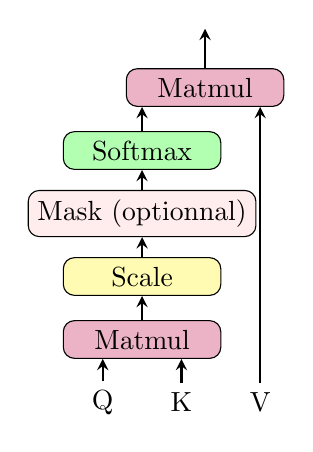
\begin{tikzpicture}[node distance=0.8cm]

\tikzstyle{matmul} = [rectangle,rounded corners, minimum width=2cm , text centered, draw=black, fill=purple!30]
\tikzstyle{softmax} = [rectangle,rounded corners, minimum width=2cm , text centered, draw=black, fill=green!30]
\tikzstyle{mask} = [rectangle,rounded corners, minimum width=2cm , text centered, draw=black, fill=pink!30]
\tikzstyle{sca} = [rectangle, rounded corners, minimum width=2cm ,text centered, draw=black, fill=yellow!30]
\tikzstyle{action} = [rectangle, rounded corners, minimum width=2cm ,text centered, draw=black, fill=red!30]
\tikzstyle{arrow} = [thick,->,>=stealth]


% Define nodes
\node (matmul1) [matmul]{Matmul};
\node (softmax)[softmax, below of = matmul1, xshift = -0.8cm]{Softmax};
\node (mask) [mask, below of=softmax]{Mask (optionnal)};
\node (scale) [sca, below of=mask]{Scale};
\node (matmul2) [matmul, below of=scale]{Matmul};
\node (q) [below of=matmul2, xshift=-0.5cm]{Q};
\node (k) [below of=matmul2, xshift=0.5cm]{K};
\node (v) [below of=matmul2, xshift=1.5cm]{V};


% Draw arrows
\draw [arrow] (matmul1.north) -- ([yshift=0.5cm]matmul1.north);
\draw [arrow] (softmax.north) -- ([xshift=-0.8cm]matmul1.south);
\draw [arrow] (mask.north) -- (softmax.south);
\draw [arrow] (scale.north) -- (mask.south);
\draw [arrow] (matmul2.north) -- (scale.south);
\draw [arrow] (q.north) -- ([xshift=-0.5cm]matmul2.south);
\draw [arrow] (k.north) -- ([xshift=0.5cm]matmul2.south);
\draw [arrow] (v.north) -- ([xshift=0.7cm]matmul1.south);



\end{tikzpicture}